\section{Model Comparison: Linear Regression vs. ZOIB}

\subsection{Dataset Characteristics}
The dataset contains 9,180 posts with divergence scores between 0 and 1. The distribution is highly skewed, with 54\% zero divergence, 1.4\% complete divergence, and a mean score of 0.188. The bounded distribution motivates the use of ZOIB regression.

\begin{figure}[!htbp]
\centering
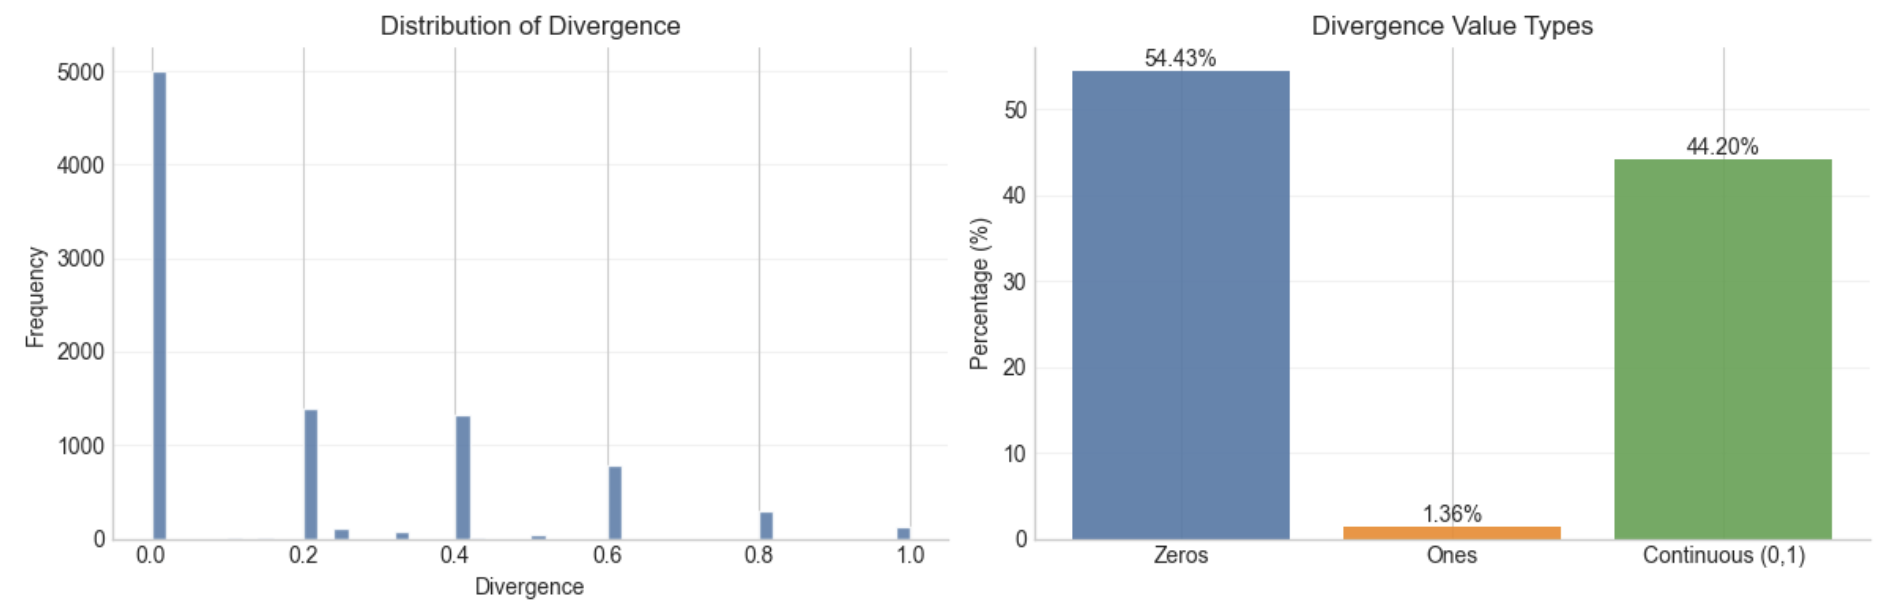
\includegraphics[width=0.8\textwidth]{plots/div_distribution.png}
\caption{Distribution of Divergence }
\label{fig:divergence_distribution}
\end{figure}


\subsection{Linear Regression}

The linear model explained approximately 34\% of the variance in divergence.
The model identified meaningful relationships:
\begin{itemize}
    \item Divergence decreases as post age increases (newer posts exhibit higher divergence).
    \item Posts with a higher total number of comments tend to show more divergence. This is intuitively correct.
\end{itemize}

However, the model shows limited predictive ability. The training and testing set prediction plots are nearly identical, indicating that the model is not overfitting and not underfitting.

\begin{figure}[!htbp]
\centering
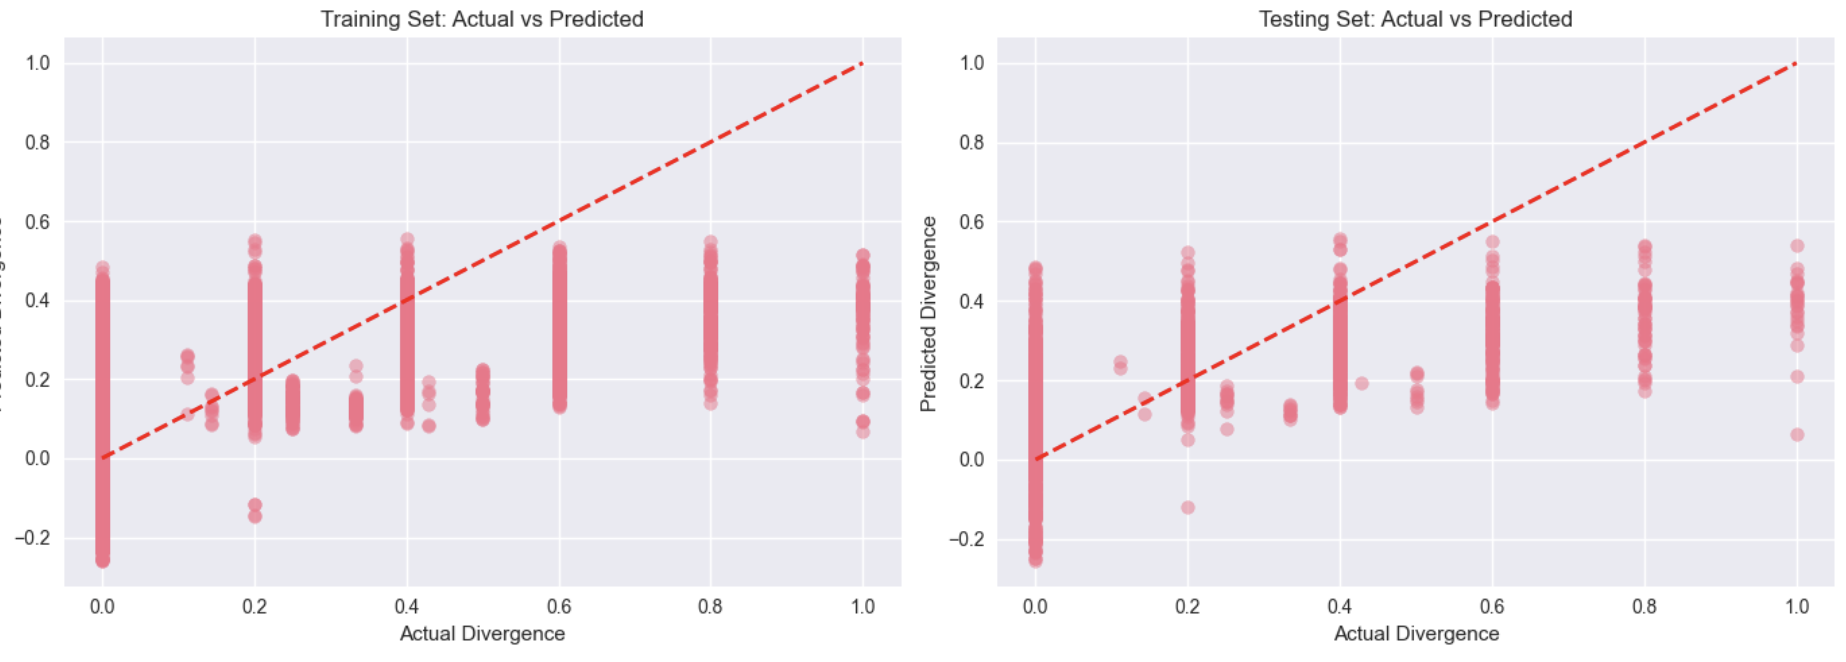
\includegraphics[width=0.8\textwidth]{plots/actual_vs_predicted_linear.png}
\caption{Actual vs. Predicted Divergence for Linear Regression}
\label{fig:linear_actual_predicted}
\end{figure}


Pairwise linear regression across all 15 user-group combinations revealed that the flat, vertically distributed pattern persists uniformly. This demonstrates that the predictive failure is not merely an artifact of grouping multiple classes, but rather stems from an inherent lack of a linear signal in the data, encouraging the use of generalized non-linear modeling and richer feature extraction to capture the underlying variance.



\begin{figure}[!htbp]
\centering
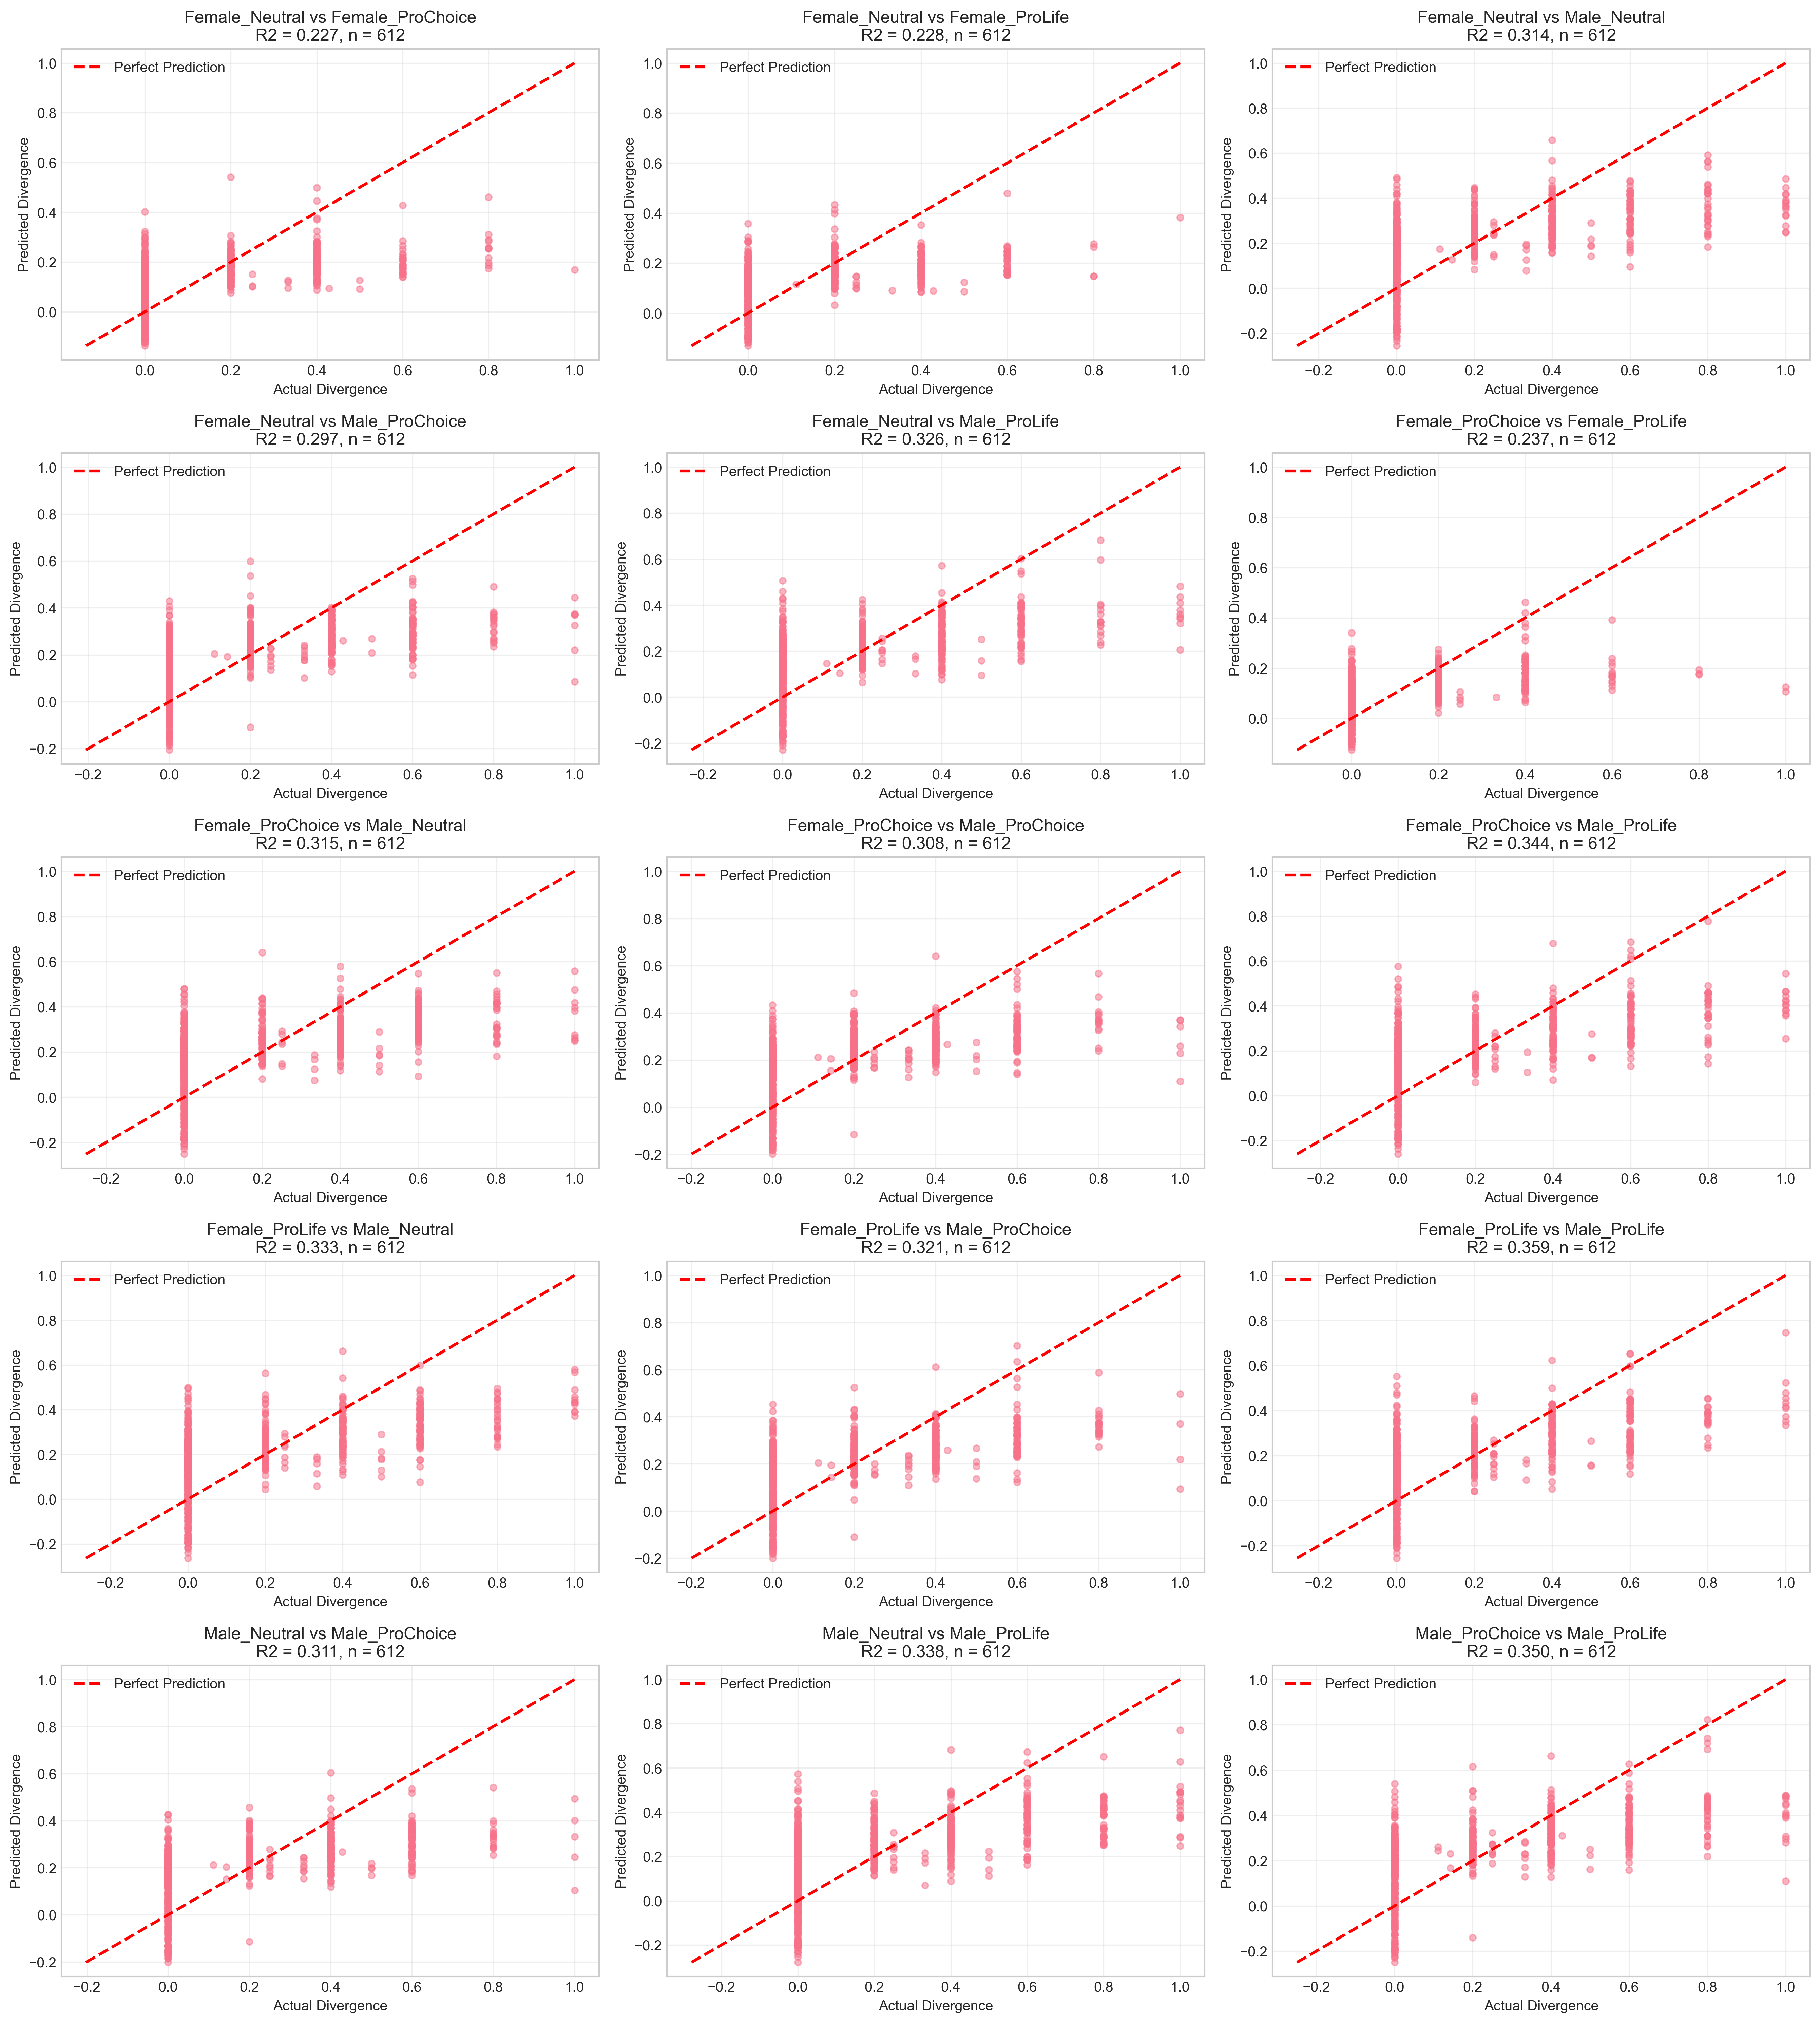
\includegraphics[width=0.8\textwidth]{plots/15_model_predictions.png}
\caption{Actual vs. Predicted Divergence for Pairwise Linear Regression Across the 15 Combinations of 6 User Groups}
\label{fig:linear_15_model_predictions}
\end{figure}

\vspace{1cm}
However, alternative approaches, Ridge, Lasso, and XGBoost, did not meaningfully improve performance. Linear regression performed the same overall, though XGBoost was slightly better but not by much.












\vspace{1cm}


\subsection{Zero-One Inflated Beta (ZOIB) Regression}

The model separates divergence into three distinct processes:
\begin{enumerate}
    \item the probability of zero divergence;
    \item the probability of complete divergence;
    \item the mean divergence for observations strictly between 0 and 1.
\end{enumerate}

The fitted ZOIB model achieved the following predictive performance:

\[
R^2 = 0.4427, \qquad
RMSE = 0.1868, \qquad
MAE = 0.1294.
\]

Compared with the linear regression model, the ZOIB model achieved a higher predictive $R^2$ (0.4427 versus 0.3472), corresponding to an approximate 28\% relative improvement in predictive performance. Because the two models use slightly different predictor sets, this improvement should not be attributed solely to the modelling framework.

\subsection{Performance Comparison}

\begin{table}[H]
\centering
\begin{tabular}{lcc}
\hline
\textbf{Metric} & \textbf{ZOIB} & \textbf{Linear Regression} \\
\hline
$R^2$ & 0.4427 & 0.3472 \\
RMSE & 0.1868 & 0.2022 \\
MAE & 0.1294 & 0.1599 \\
\hline
\end{tabular}
\caption{Predictive performance of the ZOIB and linear regression models.}
\end{table}

\subsection{Feature Interpretation}

Despite their different modelling assumptions, both approaches identified similar overall patterns.

\begin{itemize}
    \item \textbf{Time effect:} Older posts tend to exhibit lower divergence.
    \item \textbf{Engagement effect:} Higher engagement, measured by likes and comments, is associated with greater divergence.
    \item \textbf{Gender effect:} Gender matching is generally associated with lower divergence, although the ZOIB model reveals that its effect differs across the zero-inflation, one-inflation, and continuous components.
\end{itemize}

A key advantage of the ZOIB framework is that it models the mechanisms generating zero divergence, complete divergence, and intermediate divergence separately, providing a more detailed understanding of the response process than ordinary linear regression.

\subsection{Regression Analysis of Presence and Rank Variation}


To formally test which factors are associated with the observed variation, two Bayesian generalized linear mixed models with a beta-binomial likelihood were fit, one for presence variation and one for rank variation. Each observation corresponds to one post and one pairwise account comparison. Fixed effects include the log-standardized number of comments and likes on the post, the log-standardized age of the post at the time of scraping, a non-directional pairwise label for the gender combination of the two accounts being compared (female-female, female-male, or male-male), a non-directional pairwise label for the stance combination of the two accounts (e.g., prolife-prolife, prochoice-prolife, neutral-prochoice), and the political classification assigned to the post itself (pro-life, pro-choice, ambiguous, or abortion-related but not clearly classifiable to either side). A random intercept for post identity was included in both models to account for repeated comparisons drawn from the same post.
Figure 12 shows the posterior estimates for the presence-variation model. Of all the fixed effects considered, only the age of the post shows a 95\% credible interval that clearly excludes zero, with older posts consistently associated with lower presence variation. Neither the account's own gender pairing nor its stance pairing reaches a comparable level of association once post age and engagement metrics are accounted for; the credible intervals for all six stance-pair categories and all three gender-pair categories overlap zero, although the female-female category shows the most negative point estimate among the gender comparisons, consistent with the descriptive pattern seen in Figure 1. Similarly, none of the four levels of the post's own political classification reaches statistical significance in this sample.

\begin{figure}[H]
\centering
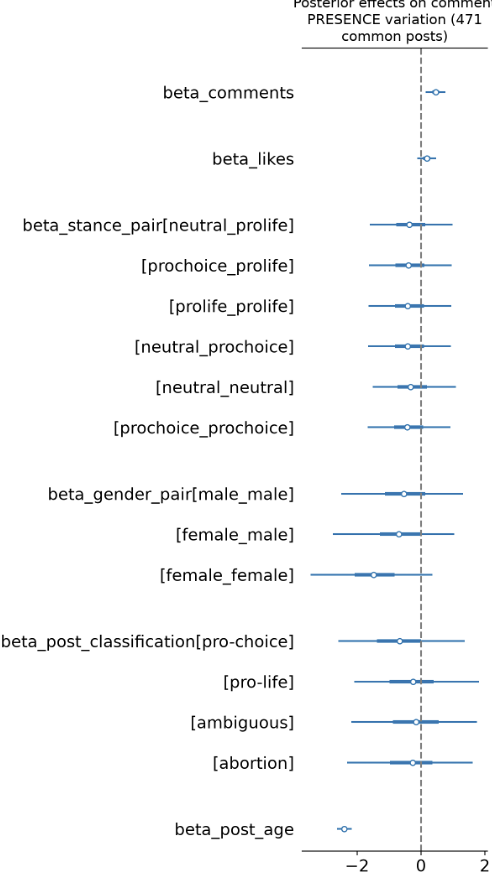
\includegraphics[width=0.8\textwidth]{plots/Posterior_effects_1.png}
\caption{Posterior effects on comment presence variation (471 common posts).}
\end{figure}

Figure 13 shows the corresponding posterior estimates for the rank-variation model. The pattern closely replicates that of the presence-variation model: post age is again the only fixed effect whose 95\% credible interval excludes zero, with the same negative direction, while comment count, like count, gender pairing, stance pairing, and the post's political classification all show credible intervals overlapping zero. As in the presence model, the female-female gender pairing again shows the most negative point estimate of the three gender categories, mirroring the female-pair pattern observed descriptively in Figure 2, though this difference does not reach statistical significance given the width of its credible interval.

\begin{figure}[H]
\centering
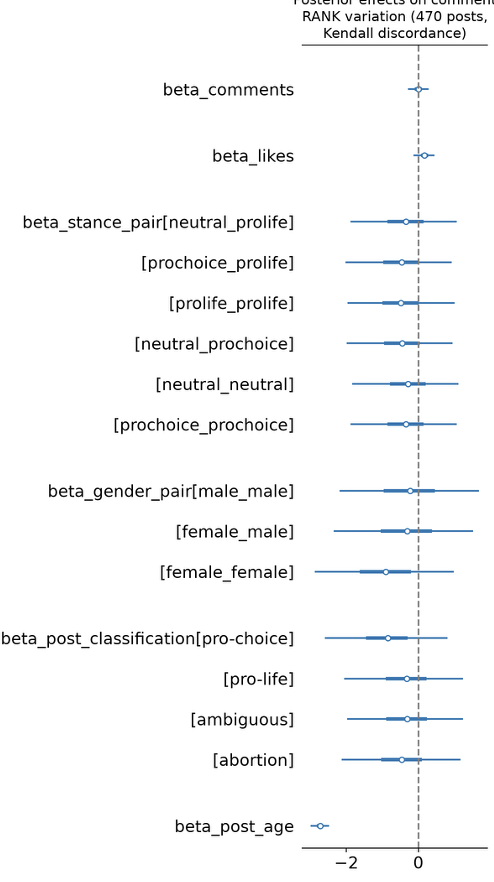
\includegraphics[width=0.8\textwidth]{plots/Posterior_effects_2.png}
\caption{Posterior effects on comment rank variation (470 posts, Kendall discordance).}
\end{figure}

Overall, the regression results indicate that post age is the only variable in either model whose association with comment variation is statistically credible, for both presence and rank-based measures. The political side of the post, the political stance of the viewing accounts, and their gender do not show a statistically credible association with either form of variation once post age and engagement metrics are accounted for, despite the visible gender-related pattern in the descriptive heatmaps.